\documentclass[conference]{IEEEtran}
\IEEEoverridecommandlockouts
% The preceding line is only needed to identify funding in the first footnote. If that is unneeded, please comment it out.
\usepackage{cite}
\usepackage{amsmath,amssymb,amsfonts}
\usepackage{algorithmic}
\usepackage{graphicx}
\usepackage{textcomp}
\usepackage{xcolor}
\usepackage{float}
\usepackage{comment}
\def\BibTeX{{\rm B\kern-.05em{\sc i\kern-.025em b}\kern-.08em
    T\kern-.1667em\lower.7ex\hbox{E}\kern-.125emX}}
    
\usepackage[style=numeric]{biblatex} %Imports biblatex package

\addbibresource{bibliography.bib}
\AtBeginBibliography{\footnotesize}
\usepackage{todonotes}
\usepackage[title]{appendix}

%%
\usepackage{lipsum}
%%

% Hyperlinking within text.
\usepackage{hyperref}
\pdfstringdefDisableCommands{%
  \def\\{}%
}

% Importing graphics and defining the graphics path
\usepackage{graphicx}
\graphicspath{{./}{./Figures/}}

\usepackage{csquotes}
\usepackage{hhline}
\usepackage{float}
\usepackage{subcaption}
\usepackage{multirow}

\usepackage{xcolor}

\usepackage{comment}
\begin{document}

\title{Accent Detection Using Deep Learning and Ensemble Methods\\

\thanks{}
\author{\IEEEauthorblockN{Finn McFall}
\IEEEauthorblockA{\textit{Engineering Mathematics} \\
\textit{University of Bristol}\\
vw19407@bristol.ac.uk}
\and
\IEEEauthorblockN{Callum Paton}
\IEEEauthorblockA{\textit{Engineering Mathematics} \\
\textit{University of Bristol}\\
eg19901@bristol.ac.uk}
\and
\IEEEauthorblockN{Leo Pitsillides}
\IEEEauthorblockA{\textit{Mathematics} \\
\textit{University of Bristol}\\
jm19052@bristol.ac.uk}
\and
\IEEEauthorblockN{Chris Sharp}
\IEEEauthorblockA{\textit{Engineering Mathematics} \\
\textit{University of Bristol}\\
zt19515@bristol.ac.uk}
}
}

\maketitle

\begin{abstract}
An accent is a distinctive way of pronouncing a language, especially one associated with a particular country, area, or social class. The motivation for automatically detecting a person's accent derives from the underrepresentation of minority groups in accent datasets. This paper uses two machine learning algorithms to investigate which approach yields better results when classifying the native language of audio files. Features from the audio files are selected using automated feature extraction and reduction processes (Surfboard and ANOVA). The features are used to train a random forest classification model, which produces a macro averaged F1 score of 0.76 for the binary model. Although, this diminishes to 0.4 when applied to a multi-class problem. The CNN is trained using the mel-spectrogram images and yields a binary macro F1 score of 0.84, and a multi-class score of 0.53. The lack of sufficient data meant the models struggled with handling multi-class problems, but the binary results demonstrate that with improved data, accent detection is feasible. Dealing with large audio files proves to be computationally expensive, so a convolutional autoencoder was implemented to extract the most important features from the image. The autoencoder provides an insight into how the project can be furthered, however, it doesn't increase the accuracy of the current model.
\end{abstract}

\section{Introduction}
\label{sec:Intro}

In the 1950s, Bell Laboratories was the first company to develop an automated speech recognition (ASR) device - capable of recognising only single spoken digits \cite{pierce1969whither}. However, huge progression in this technology empowered Apple to spearhead the ASR industry with Siri in April 2011, and Amazon soon followed suit, releasing Alexa in 2014.

These advancements in ASR technology has opened up a field of opportunities for speech pattern analysis and classification. But a common issue amongst speech recognition systems is the difficulty in detecting particular accents. This is due to under-representation of minority groups within speech archives. Often, training data is biased towards white males and people living in countries where AI technology is more advanced \cite{racistAI}. Improving the ability of AI systems to detect the nationality or accent of an individual can help to reduce discrimination and misrepresentation. As explored by Koenecke et al. in ‘Racial disparity in automated speech recognition’, there is a gap in performance on different accents when tested on five commercial ASR systems, with a bias towards white Americans \cite{SPEECH}.

In this paper, a selection of data imbalance mechanisms are introduced to increase prediction accuracy on minority classes, including creating new audio files by augmenting the original dataset. Two models are developed, a deep learning method and an ensemble approach. Both are utilised to detect an individual's accent by exploring the features and various spectrogram representations. 

Both methods will consider two classifiers, one binary for detecting American and Spanish accents and one multi-class, with French and German speakers also included. This work aims to build an ASR system that can accurately detect accents, even with an unbalanced training set, to help reduce the discrimination that currently exists in this field. 

\section{Literature Review}
\label{sec:Lit}
Accent detection is a comprehensively studied area within speech recognition and much of the work in this paper draws upon scientific literature to aid the building of the models described.

A common approach for audio classification is to convert the audio files to either Mel-spectrograms or Mel Frequency Cepstral Coefficients (MFCCs). These capture the essential features of speech and serve as a suitable input to deep learning models. They use a mel-scale that scales frequencies to be congruent with the natural auditory range of humans, emphasising high precision in the lower frequencies and low precision in the higher frequencies \cite{SimpleSpeech, MusicGenre}. The paper, ‘Deep learning approaches for understanding simple speech commands’ compares the performance of both image types on a convolutional neural network (CNN) and concludes that there is greater feature correlation with mel-spcectrograms leading to higher accuracy \cite{SimpleSpeech}. For this investigation, training will be performed on both image types.

Another approach to audio classification is to use extracted features on a random forest model. Random forests are an ensemble method designed to reduce variance and prevent overfitting of a single decision tree by using bagging and feature randomness. This is explored in ‘Speaker Recognition using Random Forest’ where different audio components are run through a random forest and their performance analysed \cite{nawas2021speaker}. For this model, pythons surfboard library is used to extract audio features from multiple components. 

\section{Method}
\subsection{Data Preprocessing}

The performance of classification tasks often comes down to the amount of training data available, and the quality of the data preparation \cite{dcgan}. Fortunately, George Mason University hosts an accent archive that contains 2140 \textit{.mp3} speech samples collected by individuals from 177 countries with 214 different native languages \cite{dataset}. Each speaker reads out the following passage in English:

\bigbreak{}

\textit{‘Please call Stella. Ask her to bring these things with her from the store: Six spoons of fresh snow peas, five thick slabs of blue cheese, and maybe a snack for her brother Bob. We also need a small plastic snake and a big toy frog for the kids. She can scoop these things into three red bags, and we will go meet her Wednesday at the train station.’}

\bigbreak{}

Alongside the \textit{.mp3} audio recordings, there is a \textit{.csv} file containing demographic information about each speaker. For this investigation, a person's accent is labelled according to their native language. For an initial binary classification model, the largest native English accent set, American, is chosen and compared to the largest non English accent set, Spanish. For the multi-class models, German and French accents are also introduced since they contain a reasonable number of files in comparison to other non-English speaking countries. Unfortunately, there is still a large disparity in class size. The full dataset used in this investigation contains 373 American speakers, 163 Spanish speakers, 64 French and 36 German.

\subsection{Dealing with Class Imbalance}

Class imbalance in machine learning leads to a bias toward majority label. To deal with this problem, several techniques are deployed. Firstly, file augmentation is used on the German and French training data, increasing the total number of samples for each class to 100. The \textit{.mp3} files are modified by altering the voice pitch and speed at random \cite{fukuda18_interspeech}. In adding the augmented files to the French and German training sets, they become less homogeneous, improving the generalisability of the model.

Two further methods of reducing imbalance are used, upsampling and class weighting. Upsampling is a simple method which equalises the distribution of classes by duplicating random samples from the training sets of all minority classes. Alternatively, a class weighting procedure can be used, where a larger weight is assigned to smaller classes. A larger class weight value means a mistake on that class is more heavily penalised.

The class weightings for each class are computed according to the following formula,

\begin{equation}
W_{j}= \frac{S}{C \times S_{j}} 
\end{equation}
where $S$ is the number of total samples, $C$ is the number of classes and $S_j$ is the total sample number for class $j$. 

Both methods of dealing with class imbalance shall be used during development of the random forest and CNN models and their effectiveness compared. 

\subsection{Random Forest Model}
In order to produce a random forest model for audio classification, first, features must be extracted. Surfboard is a Python library designed specifically for extracting features such as standard deviation and skewness from different audio components such as loudness or log mel-spectrograms. For each audio file in the dataset, a total of 19880 features are extracted \cite{surfboard}. 

To reduce the complexity of the models and eliminate redundant data, feature selection is used to extract the most informative 100 features. This is done using analysis of variance (ANOVA). ANOVA is a statistical test for determining if two sample means come from the same distribution. As explored by Wu, ANOVA for feature selection in speech recognition is computationally cheap in comparison to other methods such as SVM-RFE (Support Vector Machine – Recursive Feature Elimination) \cite{featselectionWU}. The paper also states that performance can lapse for smaller number of features and is optimal at around 100 features.

Having found the 100 best features for both the binary and multi-class classifiers, the dataset is split 70/30 into training and test sets.

To improve generalisation of the models and avoid overfitting, hyperparameters are tuned using a random search cross validation method. For each model, 100 random combinations of parameters are fitted. For each combination, the model is fit three times, with a random validation set drawn from the training set to avoid overfitting. The optimum hyperparameter combinations are those which return the highest validation macro-averaged F1 score. In the multi-class model, augmented files are removed from the training set to avoid skewing the F1 scores during cross validation. The search is also performed without the use of upsampling or class weighting. The final hyperparameters used for the model can be seen in \autoref{hyp}.

% A grid of hyperparameters values is initialised. The grid contains 10 maximum depth values from 1 to 25, 10 number of trees values from 200 to 2000, as well as options for choosing the number of features to consider when splitting. As well as the minimum number of samples required to be at a leaf node and minimum number of samples to split an internal node.

\begin{table}[H]
\centering
\begin{tabular}{|l|l|l|l|l|l|}
\hline
\textbf{Classification Method} & $\theta_1$ & $\theta_2$ & $\theta_3$ & $\theta_4$ & $\theta_5$ \\ \hline
Binary & 600 & 7 & 1 & 2 & 10 \\ \hline
Multi-class & 1400 & 7 & 2 & 2 & 10 \\ \hline
\end{tabular}
\caption{Optimum hyperparameters for the two models found using a random search method. $\theta_{1}$ is the number of trees, $\theta_{2}$ the maximum depth, $\theta_{3}$ the minimum number of features to consider when splitting, $\theta_{4}$ the number of minimum samples to be a leaf node and  $\theta_{5}$ the maximum number of features for a split.}
\label{hyp}
\end{table}


\label{sec:method}

\subsection{Convolutional Neural Network}

Training the convolution neural network (CNN) requires the conversion of each audio file into images, to then be trained on using image classification. The two graphical image representations investigated are mel-spectrograms and mel-frequency cepstral coefficients (MFFCs). When running initial models, the results on the validation set showed that MFCCs, whilst slightly less computationally expensive during training, are less accurate than the mel-spectrograms. Therefore, this model shall focus solely on classifying the mel-spectrograms. These are split 60/20/20 into train, test and validation sets.

\begin{figure}[H]
    \centering
    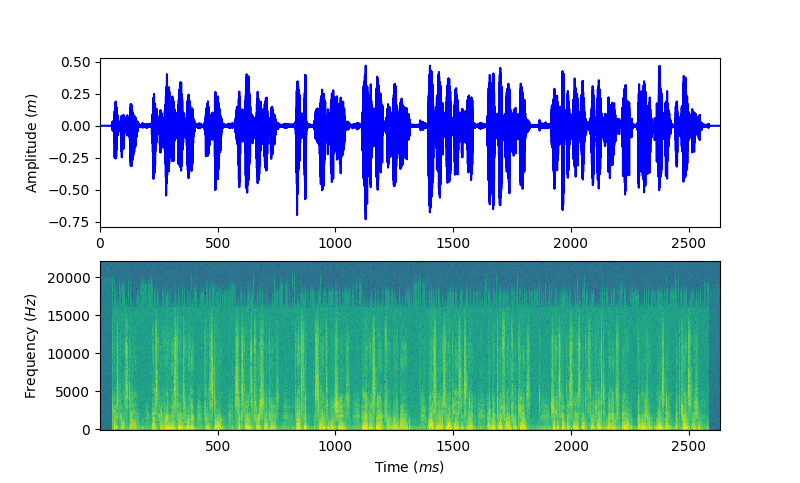
\includegraphics[scale=0.31]{Figures/WavePicture.png}
    \caption{Graphs displaying the Wave Form and Mel-spectrograms for a randomly selected American speaker.}
    \label{fig:WaveForm}
\end{figure}

Due to a shortage of data, a lower complexity CNN architecture is considered as suggested by Brigato et al in 'A close look at deep learning with small data' \cite{SmallData}. It states that, when implemented on a small dataset, low-complexity CNNs perform comparably well or better than state-of-the-art architectures. In this paper, the 'CNN-hc' architecture performed consistently well and will therefore form the base structure in this report.
%In the paper, there is consistent improvement on small datasets when implementing the `CNN-hc' architecture over competing architectures. Therefore, this structure is used as a basis for the CNN in this report. 

\vspace{0.25cm}

\noindent \textbf{Model Architecture:} \newline
The CNN architecture consists of four convolutional layers. A kernel size of $3\times3$ is implemented with a standard stride of $1\times1$. The max-pooling layers consist of a $2\times2$ stride and a $2\times 2$ pool size. The filter size doubles at every layer starting from 32, as shown in \autoref{fig:CNN_architecture}. It is processed through a feed-forward layer so the output size is consistent with the input. ReLU activation is used throughout, except in the final layer which utilises the Softmax function. To take into account bordering pixels, padding is included. The model is optimised using Adam with a learning rate of $0.0001$ as decided via manual tuning \cite{ADAM}. Adam was implemented to prevent issues faced by Stochastic gradient descent (SGD) optimisation in which the escape from saddle points is arbitrarily slow \cite{DBLP:journals/corr/abs-2107-11774}. It is also known to converge faster than SGD, although often does not generalise as well \cite{SmallData, SGDvsADAM}.

\begin{figure}[H]
    \centering
    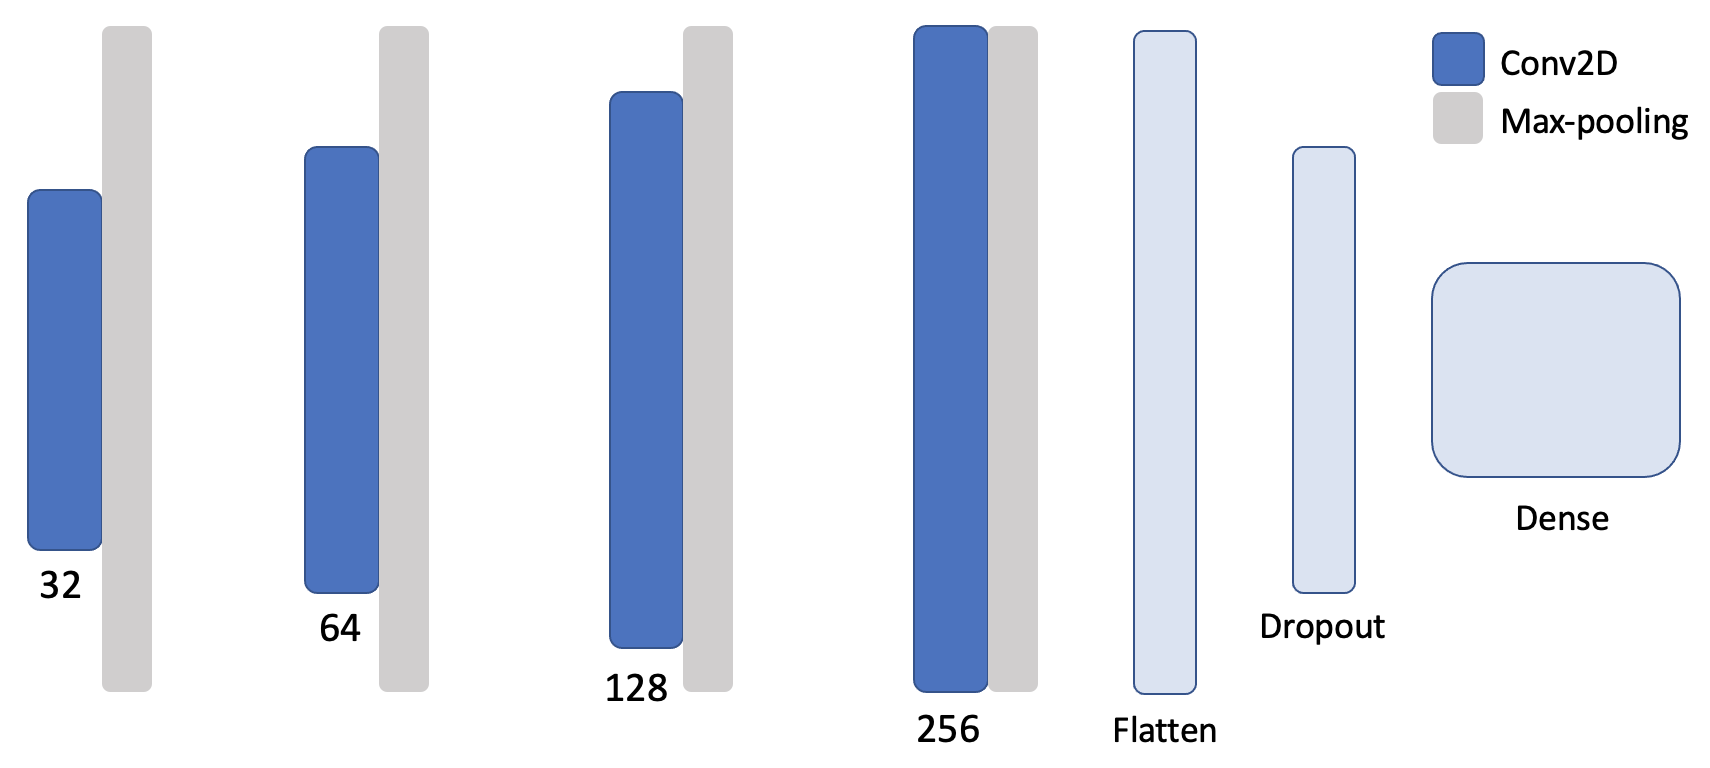
\includegraphics[width = 0.33\textwidth]{Figures/CNN_architecture.png}
    \caption{Representation of the CNN-hc architecture described by Brigato et al \cite{SmallData}.}
    \label{fig:CNN_architecture}
\end{figure}

\begin{comment}
Results in \cite{SmallData} give evidence to support the use of CNN when down-sampling but doesn't regard up-sampled or class weighted data. Given that up-sampling and class weighting will be the two methods implemented within this paper to deal with class imbalance, the table below gives a brief comparison of the different architectures on both up-sampled and class-weighted data for the binary classification task using mel-spectrograms. The results in \autoref{table:compare_architectures} show little variation between the macro F1 score for the two architectures when considering class weighted data, however, there is a clear increase in the average macro F1 score of CNN for upsampled data. As a consequence of this, and alongside the results in \cite{SmallData}, this CNN architecture will be used consistently throughout this project.
\end{comment}

\begin{comment}
\begin{table}[htbp]
\caption{F1 scores of two CNN architectures on up-sampled and class-weighted data.}
\begin{center}
\begin{tabular}{|c|c|c|c|c|}
\hline
\textbf{Country}&\multicolumn{2}{|c|}{\textbf{Up-sampled}}&\multicolumn{2}{|c|}{\textbf{Weighted}}\\
\cline{2-5}
\textbf{Pair} & mc & hc & mc & hc\\
\hline
\textbf{\textit{Usa/Spanish}} & 0.795 & 0.795 & 0.830 & 0.800
\\
\hline
\textbf{\textit{Usa/French}} & 0.705 & 0.660 & 0.625 & 0.725
\\
\hline
\textbf{\textit{Usa/German}} & 0.605 & 0.575 & 0.610 & 0.560
\\
\hline
\textbf{\textit{Spanish/French}} & 0.465 & 0.570 & 0.660 & 0.695
\\
\hline
\textbf{\textit{Spanish/German}} & 0.540 & 0.525 & 0.630 & 0.580
\\
\hline
\textbf{\textit{French/German}} & 0.465 & 0.560 & 0.600 & 0.600
\\
\hline
\textbf{\textit{Average}} & 0.596 & 0.614 & 0.659 & 0.660\\
\hline
\end{tabular}
\label{table:compare_architectures}
\end{center}
\end{table}
\end{comment}

\noindent \textbf{Regularisation:} \newline 
Due to the lack of data, the model is even more inclined to overfit. In an attempt to overcome this issue, various regularisation techniques are implemented.

Firstly, the CNN uses a dropout layer. This regularisation layer randomly omits units from the neural network along with their connections to reduce co-adaptation between units \cite{Dropout}. Brigato et al. gives evidence to support the use of dropout layers regardless of data scarcity, and produces best results using a dropout probability of $0.7$ \cite{SmallData}.

As well as this, early stopping is used to reduce both overfitting and computation time. By monitoring a chosen metric, the training process is stopped under specified conditions before the model gets the chance to overfit to the data. Optimising early stopping is highly dependent on the choice of metric and the patience parameter - the number of epochs with no improvement after which training will be stopped. It is common to use validation loss as the monitored metric especially when dealing with imbalanced data \cite{EarlyStopping}.

A large patience value prevents the model from stopping too early and hence underfitting. Thus, the patience is set to 30, meaning the network will run until there are 30 consecutive epochs with no improvement to validation loss. When this happens, weights from the epoch with the best validation loss are restored.

%Further, the early stopping class in Keras includes a parameter restore\_best\_weights which restores the weights of the epoch with the best monitored metric, in our case the validation loss.

\subsection{Convolutional Autoencoder}

In a situation where there are many more images to be trained and classified on, decreasing computation becomes more significant. Due to the size of the network and number of inputs, this is particularly important for the CNN. Each mel-spectrogram image has a shape of $456\times614\times4$, yielding an array of $1,119,936$ data points per image. An autoencoder provides a solution to this issue by learning the most relevant and discriminative features from the mel-spectrogram images as shown in \autoref{fig:autoencoder} \cite{sardari2022audio}.

%Computation time and cost proves to be a reoccurring issue within this project, especially for the CNN. The reason being both the size of the network and the size of it's inputs. Each mel-spectrogram image has a shape of $456\times614\times3$, yielding an array of $839,952$ data points per image. An autoencoder provides a solution to this issue by learning the highly relevant and discriminative features from the mel-spectrogram images \cite{sardari2022audio}.

\begin{figure}[H]
    \centering
    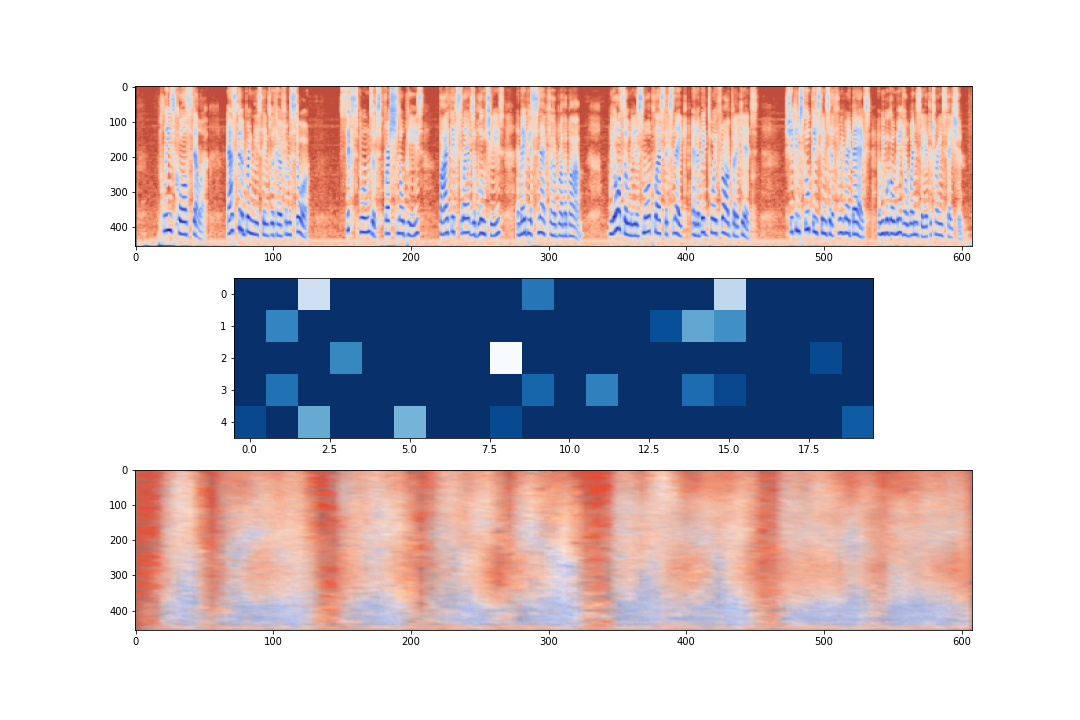
\includegraphics[scale=0.20]{Figures/Encoding.png}
    \caption{An example of a CNN-encoded mel-spectrogram image, followed by the decoded reconstruction.}
    \label{fig:autoencoder}
\end{figure}

The framework is an end-to-end CNN with two components: an encoder and a decoder. The encoder utilises several convolutional layers, followed by max-pooling layers to down sample the feature maps. It outputs a vector of 100 features, which can act as an input for another DNN or CNN for classification. The structure of the decoder follows on from the encoder and repeats it, but in reverse. The effect of this being the reconstruction of the original image from the encoding. Therefore, the autoencoder can also serve the purpose of feature extraction as well as classifying low-dimensional feature vectors, by reproducing the original image.

\section{Experimentation}
\label{exp}
Once trained and tuned, the effect of the class balancing strategies are evaluated on the validation sets. After which, the final models can be applied to the test sets and compared.

\subsection{Random Forest Experimentation}
\label{exp:rf}
Having tuned the hyperparameters of the models, they are now trained using both upsampled training data and class weighting. A validation set is then drawn from the training set and accuracy on it calculated to determine the superior method of dealing with the class imbalance. Class weighting produced better results across both the binary and multi-class models with an accuracy score of 0.77 and 0.64 respectively compared to 0.70 and 0.57 when upsampling. The upsampled training data leads to overfitting and a slight decrease in validation set accuracy in both models beyond a 50\% training set size. The learning curves for weighted classes, in \autoref{fig:LC_RF}, show how the training and validation set accuracy change with training set size.

\begin{figure}[H]
\begin{subfigure}[t]{0.241\textwidth}
  \centering
    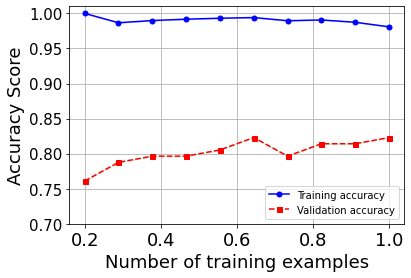
\includegraphics[width=\textwidth]{Figures/LC_binary.png}
    \captionof{figure}{Binary classifier.}
    \label{fig:binLC}
\end{subfigure}
\begin{subfigure}[t]{0.241\textwidth}
    \centering
    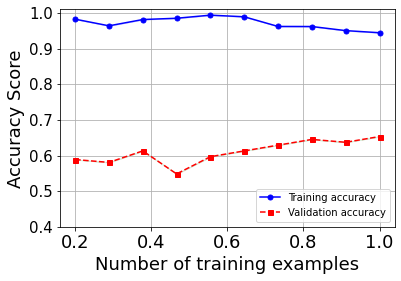
\includegraphics[width=\textwidth]{Figures/LC_multi.png}
    \captionof{figure}{Multi-class classifier. }
    \label{fig:multiLC}
\end{subfigure}
\caption{Learning curves showing training and validation accuracy using weighted classes.}
\label{fig:LC_RF}
\end{figure}

\autoref{fig:LC_RF} shows that both the binary and multi-class models do not converge to a steady validation accuracy score, inferring more data may be necessary for an improved model.
%What is also clear is the high training accuracy compared to validation accuracy. However, firstly, this is common due to the majority voting in the random forest method, and secondly, the training set contains augmented data and so correct prediction is more likely\cite{kazlou_2021}.  
%correctly for those  and so it is clear that the binary classifier has a higher accuracy than the multi-class classifier. %overfitting maybe?

%The binary classifier model converges to a validation accuracy of 0.94 when using 90\% of training data. On the other hand, the multi-class model does not appear to fully converge, suggesting more data may be necessary to optimise the model.

The final models are now used to predict the accents of the speakers in the test sets and the following confusion matrices are attained.

\begin{figure}[H]
\begin{subfigure}[t]{0.24\textwidth}
  \centering
    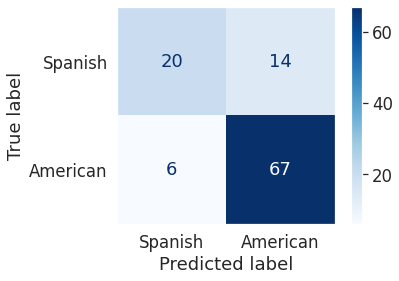
\includegraphics[width=\textwidth]{Figures/BLUE_binary_CM.png}
    \captionof{figure}{Binary classifier test set prediction.}
    \label{fig:binCM}
\end{subfigure}
\begin{subfigure}[t]{0.24\textwidth}
    \centering
    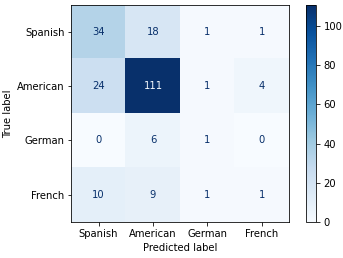
\includegraphics[width=\textwidth]{Figures/BLUE_multiclass_CM.png}
    \captionof{figure}{Multi-class classifier model.}
    \label{fig:multiCM}
\end{subfigure}
\caption{Confusion matrices of predictions for the random forest classifier model.}
\label{fig:RFCMs}
\end{figure}

The class imbalance on the test set is visible in \autoref{fig:RFCMs}. Therefore, instead of accuracy, the F1 scores for each class are computed. This is the harmonic mean of precision and recall that is used to assess performance on unbalanced data.

\begin{table}[H]
\begin{center}
\begin{tabular}{|c|c|c|c|c|c|}
\hline
\textbf{Classification}&\multicolumn{4}{|c|}{\textbf{Native Language}} & \textbf{Macro}\\
\cline{2-5}
\textbf{Method}& American & Spanish & French & German & \textbf{F1}\\
\hline
Binary & 0.83 & 0.67 & & & 0.76\\
\hline
Multi-class & 0.71 & 0.46 & 0.21 & 0.23 & 0.40\\
\hline
\end{tabular}
\caption{F1 scores for binary and multi-class classification using a random forest classifier.}
\label{tabl:RF_F1}
\end{center}
\end{table}
\begin{comment}


\begin{table}[ht]
\centering
\begin{tabular}{|l|l|l|l|l|}

\hline
    & Spanish & American & French & German \\ \hline
RF: Binary      & 0.667   & 0.825    &        &        \\ \hline
RF: Multi-Class & 0.463   & 0.713    & 0.211  & 0.232  \\ \hline

\end{tabular}
\caption{F1 scores for binary and multi-class classification using a random forest classifier.}
\end{table}


\end{comment}

\subsection{CNN Experimentation}


%As is the case with the random forest model, class weighting, specifically on the mel-spectrogram data, produces the most comprehensive results across both binary and multiclass models. 

%As expected from the various research papers[cite papers] there is a clear improvement in macro F1 score, approximately $23\%$, when implementing the CNN using mel-spectrograms over MFCCs for the class weighted data. 

From the learning curves in \autoref{fig:curves_mel_upsampled} it is evident that using class weighted data is superior to upsampled data. This is likely due to the limited window between underfitting and overfitting. Early on in the learning process the CNN begins to overfit the smaller classes because of duplicated items in the training set. On account of the detail in mel-spectrogram images, less is learnt from the training process before it is stopped due to overfitting. Without the input from early stopping to reduce overfitting, the elements, especially those in minority classes, will likely be misclassified. 
%The misclassification of minority classes contradicts the pursuit for a model that improves identification of foreign accented speakers. - good sentence but more dicussiony than results.

%However, the same is not true for the upsampled data. This is likely a result of the limited window between underfitting and overfitting. Early on in the learning process the CNN begins to overfit the smaller classes due to the duplicated elements. On account of the detail in mel-spectrogram images, less is learnt from the training process before it is stopped due to overfitting. This is evident from the learning curves in Figure~\ref{fig:curves_mel_upsampled}.
%Without the input from early stopping to reduce overfitting, the elements, especially those in minority classes, will likely be misclassified. The misclassification of minority classes contradicts the pursuit for a model that improves identification of foreign accented speakers.

\begin{figure}[ht]
\begin{subfigure}[t]{0.24\textwidth}
  \centering
    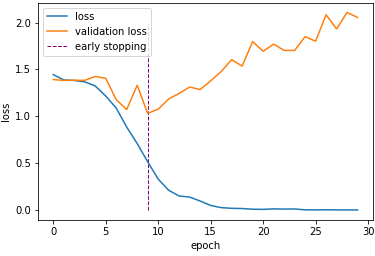
\includegraphics[width=\textwidth]{Figures/usa_spanish_french_german_mel_hc_upsampled_loss.png}
    \captionof{figure}{Loss curves of upsampled data.}
\end{subfigure}
\begin{subfigure}[t]{0.24\textwidth}
    \centering
    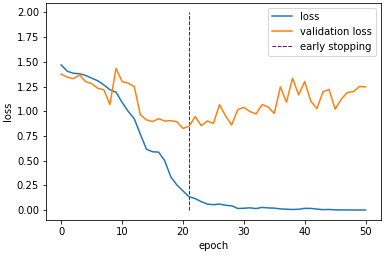
\includegraphics[width=\textwidth]{Figures/usa_spanish_french_german_mel_hc__loss.png}
    \captionof{figure}{Loss curves of class weighted data.}
    \label{fig:loss_curve_weighted}
\end{subfigure}
\caption{Learning curves comparing the overfitting of upsampled and class weighted mel-spectrogram data for multi-class classification.}
\label{fig:curves_mel_upsampled}
\end{figure}

For multi-class classification, improvement in the F1 score is observed in the upsampling method, specifically for the Spanish and German classes, however with great misclassification of at least one of the two minority classes. Given that the focus is on non-biased accent identification, this misclassification of minority classes, alongside a 51\% increase in macro F1 score, justifies the use of a class weighted sampling method for the audio classification task. A similar conclusion was gathered from the results for binary classification.

\begin{comment}
\begin{table}[ht]
\begin{center}
\begin{tabular}{|c|c|c|c|c|c|c|}
\hline
\textbf{Image} & \textbf{Sampling}&\multicolumn{4}{|c|}{\textbf{Native Language}} & \textbf{Macro}\\
\cline{3-6}
\textbf{Type} & \textbf{Method}& Usa & Spanish & French & German & \textbf{F1}\\
\hline
Mel & Upsampled & 0.84 & 0.64 &  &  & 0.74\\
\hline
Mel & Weighted & 0.91 & 0.77 & & & 0.84\\
\hline
MFCC & Upsampled & 0.91 & 0.77 &  &  & 0.84\\
\hline
MFCC & Weighted & 0.87 & 0.74 &  &  & 0.80\\
\hline
\end{tabular}
\caption{F1 scores for binary classification of American and Spanish using a CNN.}
\label{tabl:bin-class_CNN}
\end{center}
\end{table}
\end{comment}
\begin{table}[ht]
\begin{center}
\begin{tabular}{|c|c|c|c|c|c|}
\hline
\textbf{Classification}&\multicolumn{4}{|c|}{\textbf{Native Language}} & \textbf{Macro}\\
\cline{2-5}
\textbf{Method}& American & Spanish & French & German & \textbf{F1}\\
\hline
Binary & 0.91 & 0.77 & & & 0.84\\
\hline
Multi-class & 0.86 & 0.67 & 0.43 & 0.17 & 0.53\\
\hline
\end{tabular}
\caption{F1 scores for binary and mutli-class classification using a CNN.}
\label{tabl:CNN_F1}
\end{center}
\end{table}

Notice, in \autoref{fig:loss_curve_weighted}, there is clear variation is the loss between the validation and training sets indicating that the model is still overfitting. Despite attempts to overcome this issue, the cause is likely due to the lack of minority data available. This is apparent from the misclassification of minority classes in \autoref{fig:multi_CM_mel_weighted} compared to the successful binary classification of the largest two classes in \autoref{fig:bin_CM_mel_weighted}.

\begin{figure}[H]
\begin{subfigure}[t]{0.24\textwidth}
  \centering
    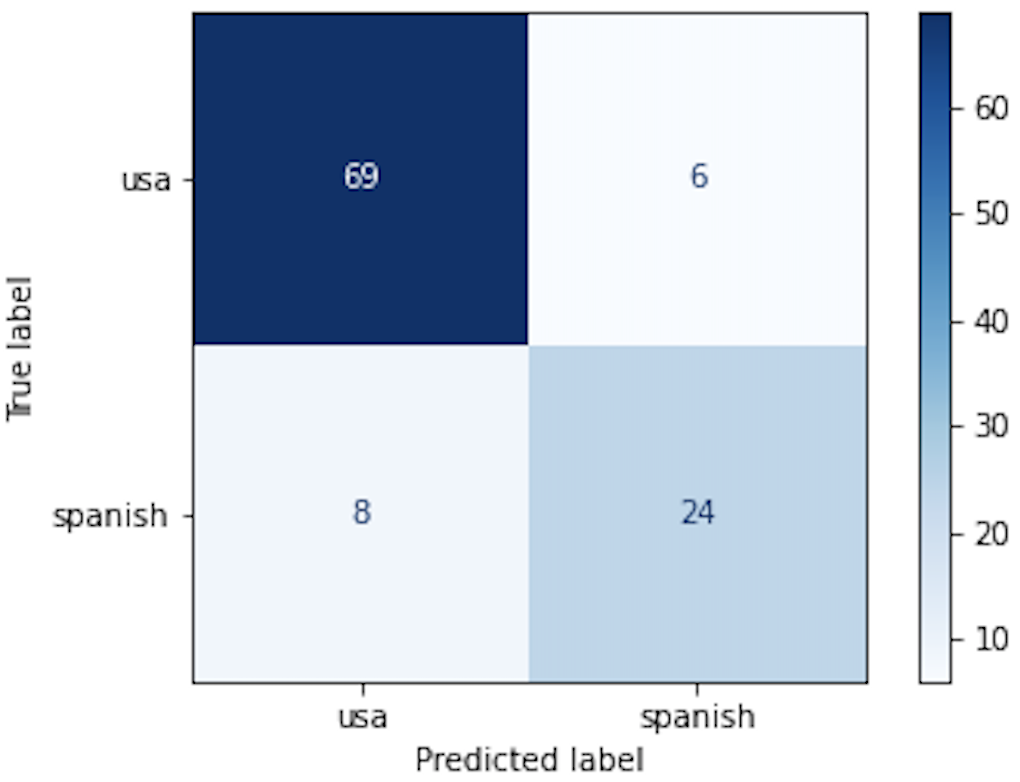
\includegraphics[width=\textwidth]{Figures/binary_confusion_matrix.png}
    \captionof{figure}{Binary classifier test set predictions.}
    \label{fig:bin_CM_mel_weighted}
\end{subfigure}
\begin{subfigure}[t]{0.24\textwidth}
    \centering
    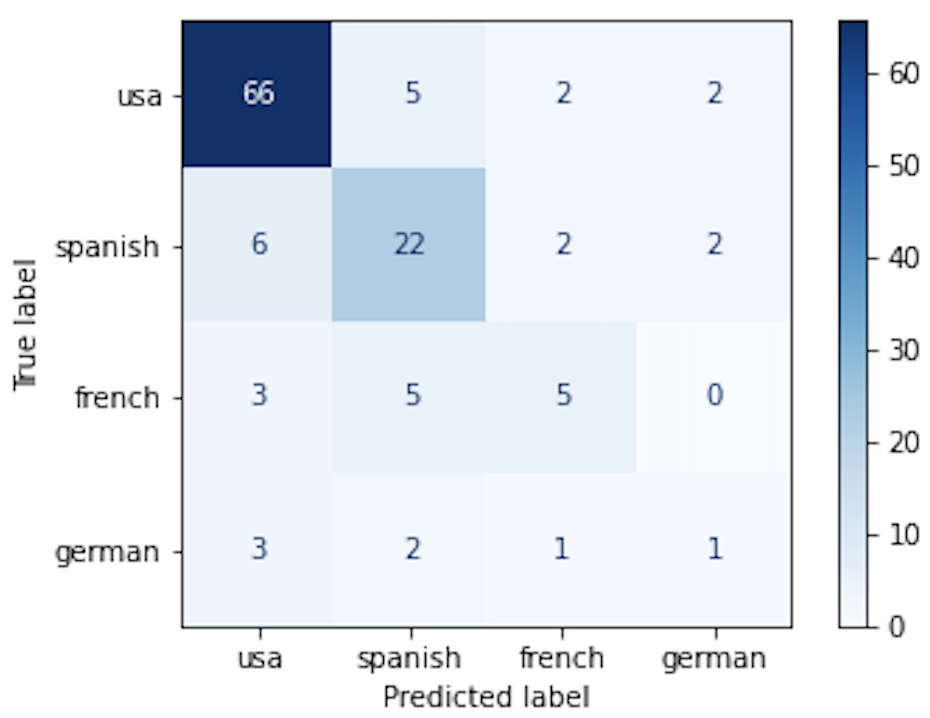
\includegraphics[width=\textwidth]{Figures/multiclass_confusion_matrix.png}
    \captionof{figure}{Multi-class classifier test set predictions.}
    \label{fig:multi_CM_mel_weighted}
\end{subfigure}
\caption{Confusion matrices of predictions for the CNN
classifier model.}
\label{fig:CNN_confusion_matrices}
\end{figure}

%ROC to represent misclassification as sample size decreases:
\begin{comment}
\begin{figure}[H]
    \centering
    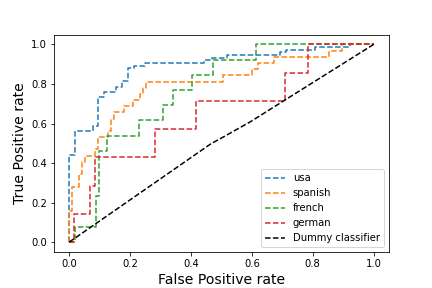
\includegraphics[width=0.5\textwidth]{Figures/ROC_CNN_multiclass.png}
    \caption{BLAH BLAH BLAH}
    \label{fig:ROC_CNN}
\end{figure}
\todo{fix caption!}
\end{comment}
\section{Evaluation}
\subsection{Model Comparison}
In order to validate the results, a dummy classifier is used as a baseline model. This uses a uniform distribution of unique classes in $y$ to generate prediction for each $x_{i}$. Now, statistical tests can be used to compare the significance of results. The \textit{5x2 paired t test} was proposed by TG Dietterich (1998) for comparing the performance of two classifiers \cite{dietterich1998approximate}. This involves splitting the dataset into 50\% training data and 50\% test data. This is repeated five times with a new random split. In each of the five iterations the F1 macro score, an unweighted average of the F1 scores of the test set, is computed. The test and train sets are then swapped leading to two different measures for each iteration, 

\begin{equation}
    p_{n}^{(1)} = F1_{A_{n}}^{(1)} - F1_{B_{n}}^{(1)}
    \quad\text{and}\quad 
    p_{n}^{(2)} = F1_{A_{n}}^{(2)} - F1_{B_{n}}^{(2)},
\end{equation}
where A and B are the two models and \textit{n} is the iteration $(n = 1,...,5)$. The mean,
\begin{equation}
    \overline{p_{n}}=\frac{p_{n}^{(1)}+p_{n}^{(2)}}{2}
\end{equation}
and sample variance,

\begin{equation}
    s_{n}^2 = (p_{n}^{(1)} - \overline{p_{n}})^2 + p_{n}^{(2)} - \overline{p_{n}})^2 
\end{equation}
is calculated and used to compute the \textit{t-statistic}. The null hypothesis ($H_0$) assumes that the the models A and B have equal performance, where model A is the dummy classifier and model B is the model being compared. Choosing a significance level of $\alpha = 0.05$, the \textit{p-value} can now be computed to determine whether the null hypothesis can be rejected. 

\begin{table}[ht]
\centering
\begin{tabular}{|l|l|l|l|}
\hline
\textbf{Model: Classification} & \textbf{T-statistic} & \textbf{P-value} & \textbf{Reject/Accept} $H_0$ \\ \hline
RF: Binary & 2.799 & 0.038 & Reject \\ \hline
RF: Multi-Class & 3.338 & 0.021 & Reject \\ \hline
CNN: Binary & 6.075 & 0.0017 & Reject \\ \hline
CNN: Multi-Class & 6.274 & 0.0015 & Reject\\ \hline
\end{tabular}
\caption{T-statistics, P-values and null hypothesis results for Random Forest and CNN, using Binary and Multi-class Classifications.}
\label{tab:T-P-Null}
\end{table}

As shown in \autoref{tab:T-P-Null}, all models developed in this paper reject the null hypothesis, meaning to a significance level of 5\%,  their performance is better than the dummy classifier results. Furthermore, the CNN produces a lower \textit{p-value} for both classifiers, this is because results were not only higher on average but also more consistent, with less sample variance. Note that the augmented data was not used for computing \textit{p-values} because replicated copies could culminate in the test set, skewing the results.
%The considerable gap in p-values between the two models is an effect of the variance of the results for the two different models.

In order to directly compare the CNN and random forest methods, ROC curves are used. These curves represent the trade off between the sensitivity and specificity to better understand the overall performance of each model on the entire dataset. To do this, the macro averaged true positive and false positive rate is calculated. This involves computing the rates independently for each class and then taking an average, thus plotting a single curve for each model. 

\begin{figure}[ht]
\begin{subfigure}[t]{0.24\textwidth}
  \centering
    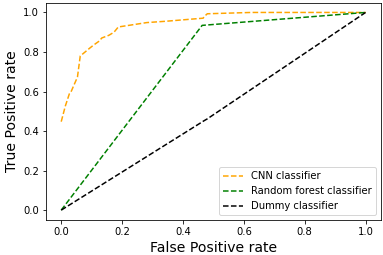
\includegraphics[width=\textwidth]{Figures/ROC_binary_macro.png}
    \captionof{figure}{Binary classification.}
    \label{fig:binROC}
\end{subfigure}
\begin{subfigure}[t]{0.24\textwidth}
    \centering
    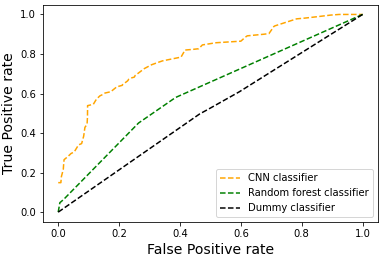
\includegraphics[width=\textwidth]{Figures/ROC_multiclass_macro.png}
    \captionof{figure}{Multi-class classification.}
    \label{fig:multiROC}
\end{subfigure}
\caption{Macro averaged ROC curves for comparison of the CNN, random forests and dummy classifier models.}
\label{fig:ROC}
\end{figure}
The area under the ROC curves can be used to assess the performance of the different models (AUC score). A perfect model would go straight up the \textit{y} axis and then along the x axis with area one, whilst a random predictor would sit on the diagonal with area 0.5. For binary classification, the CNN has an AUC value of 0.94 compared to 0.74 with the random forest model. Similarly the CNN outperforms the random forest on multi-class classifcation with an AUC score of 0.79 and 0.61 respectively.

\subsection{Discussion}
Across both the binary and multi-class classifiers, the CNN approach performed better on the test set. However, training a CNN is more computationally complex. Training both the binary and multi-class models on the CNN took over two minutes when compared to about ten seconds for the random forest models. The computational power required warrants the use of an autoencoder, which failed to improve the accuracy in this report. However, given more time, a convolutional autoencoder does have potential as a high-level feature extraction method and could be of use.

At present, both multi-class classifiers do not perform well on the minority classes. Despite the use of augmentation of training data and utilising upsampling and class weighting, class imbalance remains the limiting factor. For the model to improve, more data is required to avoid overfitting on training sets of the smaller classes. An alternative approach could be to generate synthetic audio data using a generative adversarial network, something successfully done by Madhu et al. for speech emotion recognition \cite{madhu2019data}. 

Another reason for the poor performance on the multi-class models could be that the dataset uses an English passage. As such, any non-native English speakers are likely to adopt a mock American or English accent and so detecting their natural accent becomes harder. Currently the model is more accurate when used as a binary classifier for detecting an American accent compared with a Spanish accent rather than determining the exact accent of an individual.

The lack of availability of data reflects the problems within AI about representation. This project aimed to build a model that could be used to detect accent and hence reduce the discrimination within ASR systems. However, as a result of bias within the dataset, performance on predicting a non American accent was poor. Stratified sampling of data or further development of augmentation is necessary to reduce this bias and improve the models. 

\begin{comment}
From the deployment of the two models, it is clear they obtain similar accuracy through the comparison of their F1 scores. However, the CNN is slightly better at classifying than the Random Forest model. Moreover, both methods are statistically better than an implemented dummy model. Looking at the F1 scores of the CNN-mc and CNN-hc architectures, no one structure was better than the other. Perhaps with more testing, one will prevail.

Specifically for Random Forest, extracting the full list of features from the dataset takes approximately five seconds for each file, so for a larger set it may take a significant amount of time to produce the features. However, once the best features have been selected with ANOVA, training and testing takes less than 10 seconds total. For the CNN, it takes a longer time to train and test, but does not need to extract features. 

For both models, once they have extracted the relevant features and trained on the selected data, the testing is relatively quick to perform, but as the number of files increase, the time taken the train increases. 

At early stages of model development, the models worked better at detecting whether the speaker was a native or non-native speaker. The main reason for this is because many of the non-native speakers in Europe use similar TV-shows and films to learn English. Therefore, this causes the difference between each of the non-native classes to be less than the difference between native speakers and all the non-native speakers combined. Hence when binary classification was replaced by the current multi-class classification, the accuracy and precision of the models decreased.
\end{comment}

\section{Conclusion}
\label{Conc}
This report shows the development of two separate machine learning methods, a CNN that performs image classification using mel-spectrograms and a random forest ensemble method that uses features extracted from the audio files using surfboard. Across both binary and multi-class methods, the CNN scored an 18\% higher average macro F1 score. If the project were to be taken further, it is the CNN methodology that has greatest potential, potentially incorporating the autoencoder to decrease computation time for larger datasets.  

The model as it is, is best at detecting American speakers, with an F1 score of 0.94 and 0.83 on the binary CNN and random forest classfiers respectively. However, performance on each accent in the multi-class model drops significantly due to class imbalance. Class weighting was determined to be more effective than upsampling at dealing with this. However for the multi-class models to be useful, further training with more data is required. 
The paper aimed to help improve accent detection of ASR systems in order to reduce discrimination. Although the methods described could be developed to achieve this goal, at its current state, the lack of data available for non American accents limits its effectiveness.


\printbibliography

\end{document}